%!TEX root = ../paper.tex

\begin{figure}[!ht]
\centering
\noindent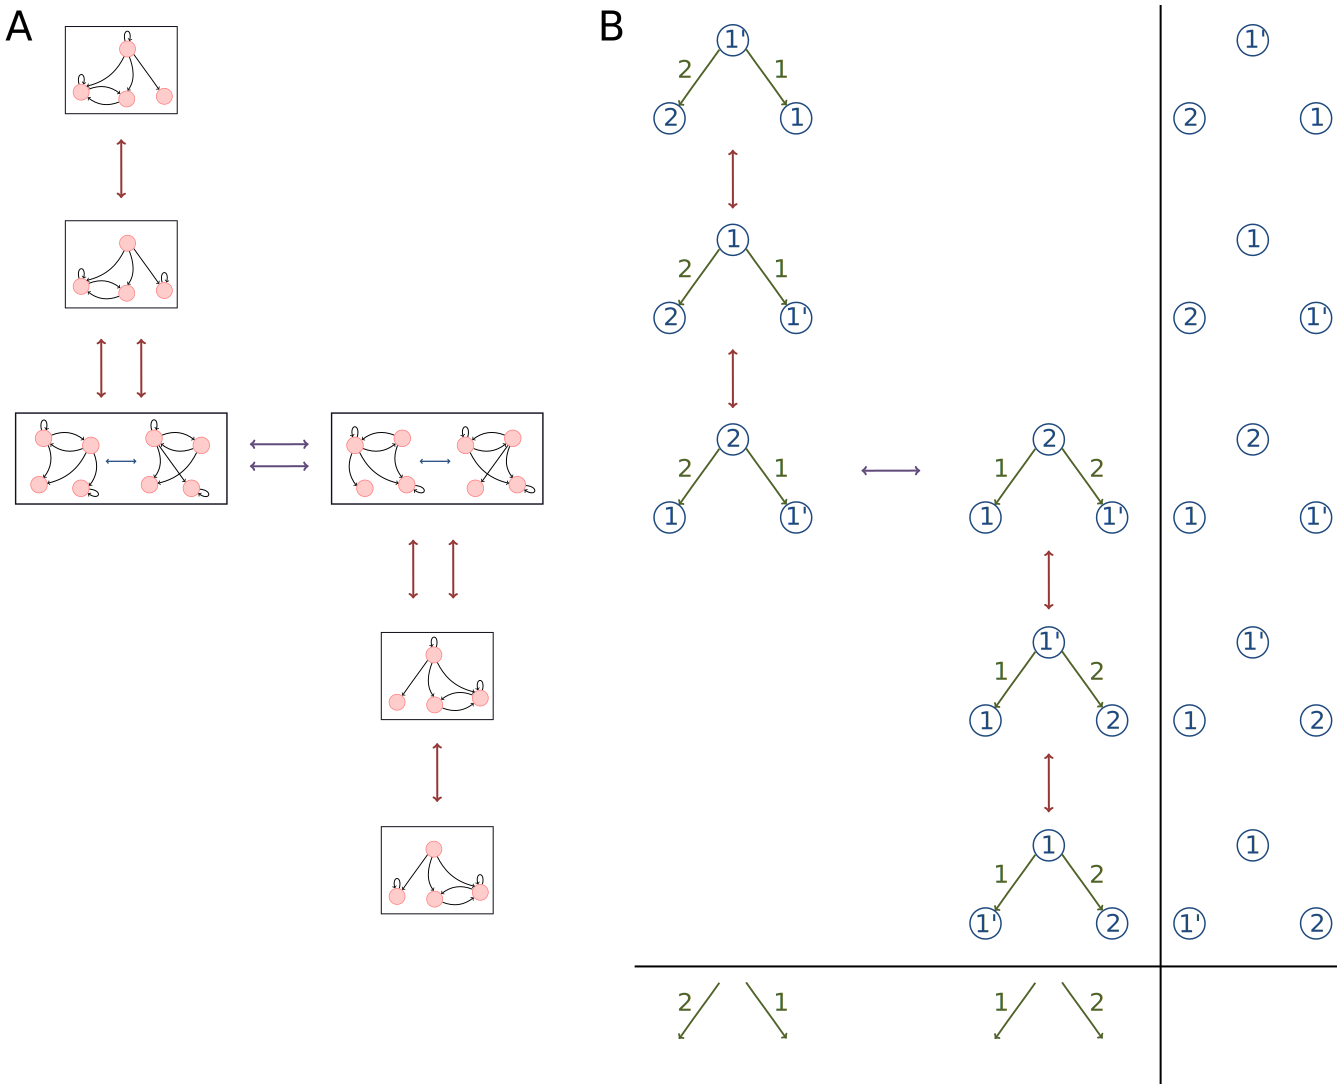
\includegraphics[width=0.9\columnwidth]{fig/robustnesssymmetries.pdf}
\caption{{\bf Example symmetries of robustness.} In this example, the connected component sizes are fixed at $\{2,1,1\}$ with a total of $3$ links between them. Red arrows correspond to transformations like \reffighiertransformations a where SCCs are swapped whereas purple arrows correspond to transformations like \reffighiertransformations b where links are moved between nodes within a SCC. (A) shows all underlying graphs while (B) shows the number of nodes in each SCC and the number of links between the SCCs.}
\label{fig:robustnesssymmetries}
\end{figure}

\pagebreak

\begin{figure}[!ht]
\centering
\noindent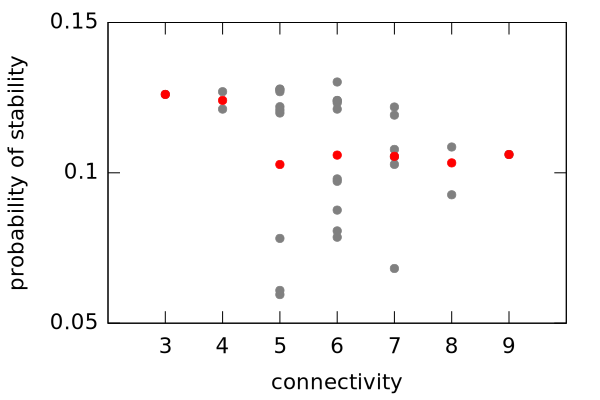
\includegraphics[width=0.8\columnwidth]{fig/apstab3x3.pdf}
\caption{{\bf System stability as a function of connectivity.} The red points represent the average of system stability at each connectivity.}
\label{fig:apstab3x3}
\end{figure}

\pagebreak

\begin{figure}[!ht]
\centering
\noindent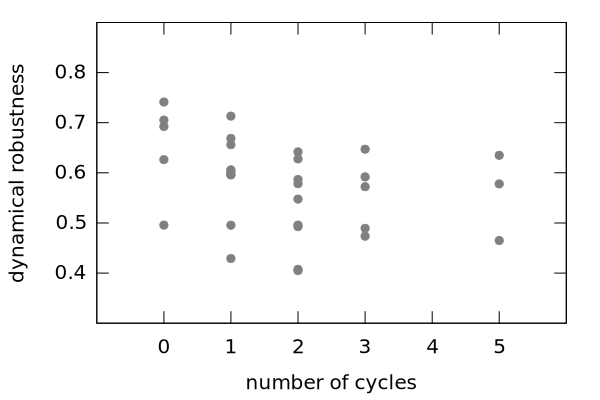
\includegraphics[width=0.8\columnwidth]{fig/cycle3x3.pdf}
\caption{{\bf dynamical robustness as a function of number of cycles.} }
\label{fig:cycle3x3}
\end{figure}

% \begin{figure}[!ht]
% \centering
% \noindent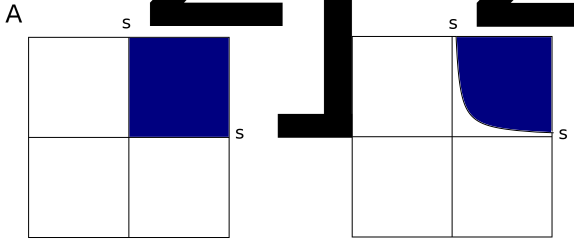
\includegraphics[width=0.7\columnwidth]{fig/region2and3.pdf}
% \caption{{\bf Stability conditions on coefficients of the characteristic polynomial for two and three component systems.} The regions correspond to all possible relationships between the invariants determined by the characteristic polynomial.}
% \label{fig:region2and3}
% \end{figure}

% \pagebreak

% \begin{figure}[!ht]
% \centering
% \noindent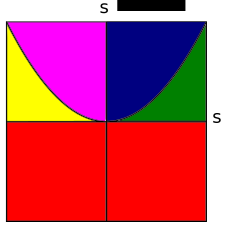
\includegraphics[width=0.5\columnwidth]{fig/region2x2.pdf}
% \caption{{\bf Stability conditions on coefficients of the characteristic polynomial for two component systems.} The regions correspond to all possible relationships between the invariants determined by the characteristic polynomial. Colors correspond to the regions given in the main text Green: $R_{2000}$, Red: $R_{1100}$, Yellow: $R_{0200}$, Magenta: $R_{0002}$, Blue: $R_{0020}$.}
% \label{fig:region2x2}
% \end{figure}

% \pagebreak

% \begin{figure}[!ht]
% \centering
% \noindent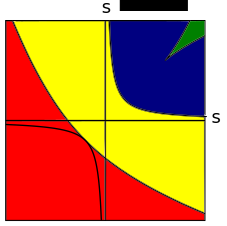
\includegraphics[width=0.5\columnwidth]{fig/region3x3.pdf}
% \caption{{\bf Stability conditions on coefficients of the characteristic polynomial for three component systems.} Colors correspond to the following regions Green: $R_{3000}$, Red: $R_{1200}$, Yellow: $R_{1002}$, Blue: $R_{1020}$. This is the plane $s_3=1$.}
% \label{fig:region3x3}
% \end{figure}
